\documentclass{fast-nuces-bs}

\usepackage{blindtext}
\usepackage{mathptmx}% Times Roman font
\usepackage[T1]{fontenc}
\usepackage{lipsum} 
\usepackage{sectsty}
\usepackage{tikz-uml}
\usepackage{titlesec}
\usepackage{refstyle}
\usepackage{booktabs} 
\usepackage{graphicx}
\usepackage{multirow}
\usepackage{color, colortbl}
\definecolor{Gray}{gray}{0.9}
% Information about the Thesis 
% -----------------------------------------------------------------------------
% (All are compulsory, do not delete any line other than author Information)
% For e.g., usually there are 3 students in a group, so leave authorone, 
% authortwo, and authorthree, and delete authorfour.
%%%%%%%%%%%%%%%%%%%%%%%%%%%%%%%%%%%%%%%%%%%%%%%%%%%%%%%%%%%%%%%%%%%%%%%%%%%%%%%
\department{Department of Computer Science}
\faculty{Computer Science}
\degreeyear{2018}
\degreemonth{December}
\degreename{Computer Science}
\campuscity{Peshawar}
\authortwo{Muhammad Arslan}{P15-6085}
\authorthree{Abdul Moiz Rana}{P15-6091}
\authorone{Muhammad Nafeel Rasheed}{P15-6010}
\supervisor{Dr. Mohammad Nauman}
\sessionduration{2015-2019}

\deanname{Dr. Hasina Khatoon}
\directorname{Dr. Tariq Khan}
\hodname{Dr. Omar Usman Khan}
\fypcoordinatorname{Shakir Ullah}
\title{A Blockchain Based Web Portal For Whistle-Blower Against Illegal Activities}
%%%%%%%%%%%%%%%%%%%%%%%%%%%%%%%%%%%%%%%%%%%%%%%%%%%%%%%%%%%%%%%%%%%%%%%%%%%%%%%

%%%%%%%%%%%%%%%%%%%%%%%%%%%%%%%%%%%%%%%%%%%%%%%%%%%%%%%%%%%%%%%%%%%%%%%%%%%%%%
% Former document starts below this
\begin{document}

\begin{acknowledgements}
	We might want to express our most profound gratefulness to every one of the individuals who gave us the likelihood to finish the Final Year Project I. An extraordinary appreciation we provide for our Final year project supervisor,  Dr. Mohammad Nauman whose commitment in animating recommendations and consolation, helped us to facilitate what's more, whose have put his full endeavours in controlling our group in accomplishing the objective which is our venture. 
	
	Moreover we might likewise want to recognize with much thankfulness the vital job 
	of the Head of Department Computer Sciences Dr. Omar Usman Khan, who gave the all 
	required and the fundamental recommendations, inspiration and support to finish the 
	undertaking  \emph{"A Blockchain Based Web Portal For Whistle-Blower Against Illegal Activities"}. We need to welcome the direction given by Evaluators, different chiefs and in addition the entire board particularly in our venture introduction that has enhanced our introduction aptitudes on account of their remark furthermore, advices. We might likewise want to extend our most profound appreciation to every one of the individuals who have 
	straightforwardly and in a roundabout way particularly our colleagues and colleagues itself, have made profitable remark recommendations on this proposition which gave us a motivation to make strides our venture.
\end{acknowledgements}

\begin{abstract}
A Whistle-blower is a person who comes forward and shares his/her knowledge on any kind of misconduct happening in his nearby surroundings.Nowadays corruption is getting gigantic at Government level in Pakistan. You never know who is indulge and at which level, going to Police or some concerned authorities is also not a wise option.So Whistle-blower, a web based platform motivates you to step ahead for the falsification in a secure way. 

The Smart Contract – An electronic contract in the Blockchain application where the trade is happening when whistle blower reports something and gets rewarded. The Police will submit both cases and evidence against any case uploaded by any whistle blower or any other police officer. Can view both cases and evidence of any region in the country.People will see all the cases up and running currently. If you have anything against any case you have to register on a whistle blower page.The Whistle-Blower instead of real name or anything they will register through a wallet number. Keeping them unknown to the police and everyone on the system. They can submit both the cases and  evidence against any case.The Agency/Judge will keep an eye on the cases and officer assigned to that case. Reward them both officer and  whistle blower for successful closing of the case in form of Cryptocurrency.
\end{abstract}

\chapter{Preliminaries and Introduction\label{sec:introduction}}

\section{Introduction}
The theme of our idea is to use most advance technology and the naïve and good people of our country together as a whistle-blower to save the country from crime.  The main focus of our system is to ensure the safety of the whistle-blowers. Because increase in crime day by day we don’t know who is corrupt or not in the system.\\
The focus on blockchain technology is to make people unknown to each other in this application of ours. Which will ensure the safety of the people real time. The cases can be of any region all around the country. People can view all the cases and if you have something regarding that case you can go and register as a Whistle-Blower and submit the evidence regarding that case which will be viewed by the Police and Jury. Once the assessment has been made, can perform execution.\\
The Police Officer and Whistle-Blower both are unknown to each other. And both will be rewarded.   The figure below (see \figref{tst}) shows an example of Whistle-Blower.\\
\begin{figure}[h]
	\centering
	\includegraphics[scale=0.40]{figures/01.png}
	\caption{Whistle-Blower}
	\label{fig:ist}
\end{figure}
 The working or idea of this project \figref{ist} is that a whistle-Blower go to the website and submit those cases that are not been already upload that shown in figure.
\begin{figure}[h]
	\centering
	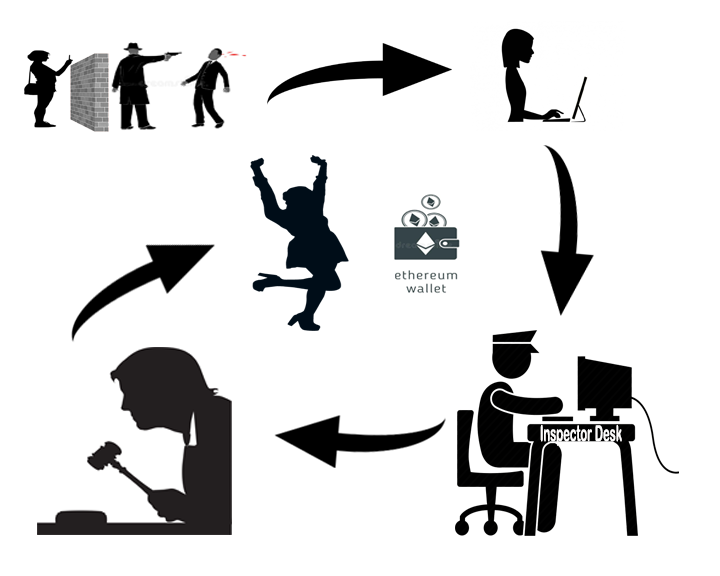
\includegraphics[width=0.50\textheight]{figures/02.png}
	\caption{Overview of Whistle-Blower}
	\label{fig:tst}
\end{figure}
In the \figref{tst}, we have Whole \textbf{ Overview } of the Whistle-Blower project that insure the security of the Person who become part of our project.\\

\subsection{Cases}
Currently we are only dealing with CORRUPTION cases only, but the system should be robust enough to accommodate other crimes in the future. The biggest challenge with the system in place is lack of rewarding mechanism and that cases are mostly mishandled and investigators are easily compromised by the perpetrators, once investigators are compromised they end up tampering with evidence and later on claiming that there wasn’t sufficient evidence. They also use delay tactics to buy time till the members of the media and members of the public has forgotten about the cases (with a work-flow based blockchain system, every step of the case will be in the public Domain and the system can even generate automated reports to show the duration each case has been at a certain stage). The investigators also start blaming the judiciary for poor verdict after cases have dragged for years and years yet mostly it’s them who door a poor job in collecting evidence. That’s why it’s important to have a system that keeps checking what’s happening at every stage of the case and who has failed the country in the fight against corruption. Rewarding mechanism is also key to make sure that there’s incentive to investigators and whistle blowers.\\
Sub categories within corruption related crimes include the following:
\begin{itemize}
	\item Conflict of interest Info / Explanation Conflict of interest
	\item  Bribery Info / Explanation Bribery
	\item  Fraud Info / Explanation Fraud
	\item  Land grabbing Info / Explanation Land grabbing
	\item  Breach of trust Info / Explanation Breach of trust
	\item  Tax evasion
		
\end{itemize}
The system should be able to assign cases to specific investigators/police based on certain rules set in the system. Investigators/police should only see cases they are dealing with or cases assigned to them. This will ensure that investigators can be held responsible for every aspect of the case without blaming their colleagues if investigation is compromised at some point.
\subsection{Corruption Sub Categories Include}
\subsubsection{Conflict Of Interest}

A conflict of interest is a situation in which a public officer has a private interest in a matter that concerns his office and he fails to disclose the private interest to his employer.
It is not an offense if the public officer has disclosed his interest and has been allowed to participate in the decision making process.\\
Some examples:\\
Self-dealing: A public officer doing a business with an organization which he works for without disclosing
Outside employment: Somebody holding two jobs in which the interest of one job conflicts with the other without disclosing

A public officer employing or giving services to a family member, relative or friends without disclosing
Gifts: Gifts from friends who also do business with the person receiving the gifts without disclosing (Such gifts may include things of value such as transportation and lodging).


\subsubsection{Bribery}
Giver: To promise, offer, or give something of value to a person in order to obtain services or gain influence; or\\
Recipient: To receive or demand, or agree to acquire or ask a private benefit so as to provide public services/goods.\\
Private benefit: gift, loan, fee, reward, appointment, service, favor, failure to take action, promise or other consideration or advantage.\\
Some examples:\\
Offering / Giving something of value
Agreeing to offer / give something of value
Demanding for / receiving a private benefit
\subsubsection{Fraud}
The action or instance of deception for financial or personal gain or so as to obtain goods or services illegally.\\
Some examples:\\

\begin{itemize}
	\item Conversion of organization’s property for personal use
	\item Falsification of documents
	\item Over valuing or under valuing of goods
	\item Conversion of organization’s property for personal use
\end{itemize}

\subsubsection{Abuse of Office}
A person who uses his office to improperly benefit oneself or another person.\\
Some examples:\\
\begin{itemize}
	\item breach of procurement rules to favour somebody
	\item Nepotism
	\item favouritism
	\item abuse of discretion / power
	
\end{itemize}

\subsubsection{Land Grabbing}
Fraudulent acquisition and disposal of public land. This includes to illegally acquire, sell, transfer, lease, charge or mortgage OR in any way dispose of public land.\\
Some examples:\\
Land set aside for public utilities such as\\


\begin{itemize}
	\item schools
	\item dispensary/hospitals
	\item road reserves and parking bays
	\item public toilets
\end{itemize}



\subsubsection{Breach of Trust}
Failure to honour a responsibility of trust and confidence bestowed upon a person by virtue of his office.\\
Some examples:\\
\begin{itemize}
	\item Where managers of pension funds have irregularly invested member funds in breach of laid down regulations
	\item Irregular investment of public funds in breach of regulations
	\item Mismanagement by appointed administrators and executors of property entrusted under their care
	\item Mismanagement of property by receiver managers / liquidators etc.

\end{itemize}



\subsection{Selected Use Cases of Application}
The main feature of our application is:
\subsubsection{Registration of Whistle-Blower}

The whistle-blowers are going to register to our system using a wallet number. If you don’t have a wallet number you can go to any crypto currency site and get one. If you want to use fiat currency, scatter wallet is also a good option. Using online wallets is because they does not trace back to you easily. Once the whistle blower is registered its wallet number will be shown only to the Jury. He/she will submit the evidence and that’s it. They also cannot see the evidence that’s already been there uploaded by the other people.
   
\subsubsection{Registration of Police Officer}

The registration of Police Officer will also be done by the same process. A wallet number and the police ID number original given by the Police Department will be used to register. If the case is uploaded by the police officer and also in his jurisdiction, he is the in charge of that case else we have to look for the regional officer where the incident happen.  

\subsubsection{Submission of Evidence/Case by Whistle-Blower/ Police Officer}
There is a general interface view of all the running cases. A criminal can also see that. But he can also be a whistle blower and see the evidence against that case. That’s why we have removed jurisdiction of anyone except police and jury to see the evidence. You can only submit the evidence and case. Cases and evidence both can be uploaded by anyone in the country. 

\subsubsection{Agency/Judge monitoring them both}
To avoid corruption and crime completely, we are introducing the jury system which will monitor the both the cases and the evidence and ask questions that what is the progress on that case. The jury will be selected very carefully and there will be more than one person so they cannot be bought. 
\subsubsection{Pending Cases}
The duration will be assigned to every single case. If the cases are older than three month, they will be shown on a separated case. 
\subsubsection{A Reward System}
If the evidence or case submitted by the police or whistle blower and finished successfully, both the police officer and the whistle blower will be awarded. These is a kind of small amount in the form of a currency. 


\subsection{How This will solve the problem through use of the blockchain}
The solution applies blockchain technology to overcome many problems around the cost, flexibility, and scalability of business support systems faced by old crime reporting systems, and to provide extensive opportunities to enhance product offerings and whistle blower experience. \\
A shared view – The Police and Judge both parties can inspect the cases fully and perform queries. People can search on the basis of region, categories, age of the case. \\
New cases and evidence – It has the ability to handle large amount of data. Its blockchain back end so if memory runs out we can simply use external cloud storage like IPFS. \\ 
Easy Reward – The Police Officer and whistle blower will be rewarded through a wallet ID by the jury.  \\
Easy and instant secure payments – The payments done will be 100 perent secure no traces back to its original owner, ensuring the safety of all the whistle blowers.   \\
A scalable solution – freeing the billing and contracting processing from physical hardware and constraints significantly improves the Operators ability to scale to explore new expansion opportunities. \\
The flexibility to respond to changing conditions – the contract mechanism give the administrator and jury the ability to change the contract to meet new upcoming challenges. \\ 
Confidential and secure client contracts – Using consortium blockchain technology i.e. per-missioned and private decentralized ledgers, the data submitted will be 100 confidential.\\ 
Secure communications – The DApp shall be securely connecting the Smart contract with the Police and whistle blower interface.  


\chapter{Blockchain\label{sec:Blockchain}}

\section{What is Blockchain}
Blockchain advancements isn't simply just single one strategy, however contains Cryptography, science, Algorithm and financial model, consolidating shared systems and utilizing circulated agreement calculation to take care of conventional appropriated database synchronize issue. \\
"Blockchain is a shared innovation, rundown of developing information put away on a conveyed record."
The figure below (see \figref{istw}) shows an example of Blockchian.
\begin{figure}[h]
	\centering
	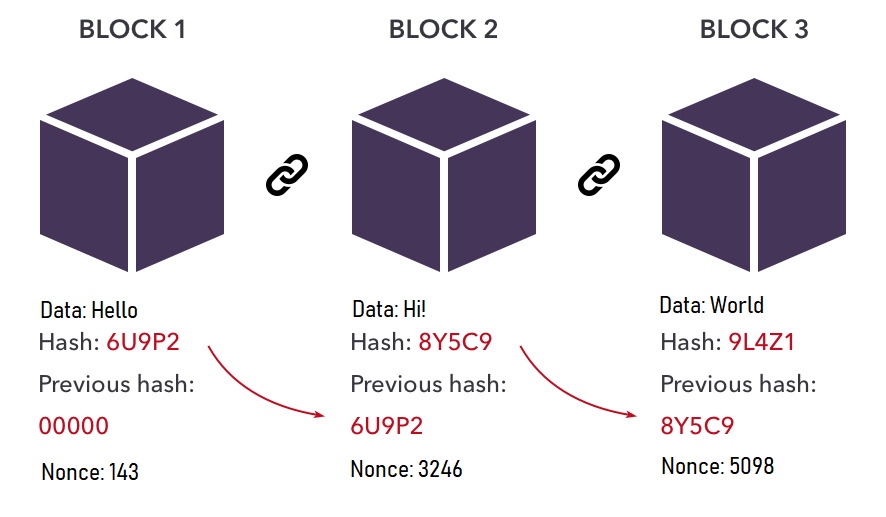
\includegraphics[scale=0.40]{figures/03.png}
	\caption{Blockchain }
	\label{fig:istw}
\end{figure}

\section{Why Blockchain}
\textbf{ De-centralised  }-Information is put away on each and every friend and nobody can adjust it. The hash of your information is created to make variability incomprehensible. Which means an advanced unique mark of your information is made. The blockchain organize is on a very basic level strong and has no-single defenselessness for programmers to abuse.\\
\textbf{ Distributed Ledger  } –Each hub (organization board) approaches the information. We will choose peers who will acknowledge or dismiss at whatever point an exchange occurred (activity made on the blockchain arrange). Means they need to achieve an agreement.\\
\textbf{ Secure  } – The information is put away after some calculation is performed on it. Hashes are created. Means permanence. Put away on various companions never alterable. \\ 
\textbf{ Transparent  } - The information's record by blockchain framework is straightforward to every hub, it additionally straightforward on refresh the information, which is the reason blockchain can be trusted.\\ 

\subsection{Hyperledger }
Their attention is on building up a measured structural system for big business class conveyed records. This incorporates distinguishing normal and basic parts, giving a practical deterioration of a venture blockchain stack into segment layers and modules, institutionalizing interfaces between the segments, and guaranteeing interoperability between records.

\subsection{Introduction Business Blockchain} 
Prerequisites shift. Adaptability, classification, consistence, work process unpredictability, and even security necessities contrast definitely crosswise over businesses and employments. Every one of these prerequisites, and numerous others, speak to a conceivably remarkable advancement point for the innovation. \\
The Hyperledger Architecture has recognized the accompanying business blockchain parts:\\
\textbf{ Consensus Layer   }-In charge of producing a concession to the request and affirming the accuracy of the arrangement of exchanges that comprise a square.\\
\textbf{ Smart Contract Layer   }-In charge of preparing exchange asks for and deciding whether exchanges are legitimate by executing business rationale.\\
\textbf{ Communication Layer   }-In charge of preparing exchange asks for and deciding whether exchanges are legitimate by executing business rationale.\\
\textbf{ Data Store Abstraction   }-Permits distinctive information stores to be utilized by different modules.\\
\textbf{ Crypto Abstraction    }-Permits diverse crypto calculations or modules to be swapped out without influencing different modules.\\
\textbf{ Identity Services   }-Empowers the foundation of a base of trust amid set-up of a blockchain occasion, the enlistment and enrollment of characters or framework elements amid system task, and the administration of changes like drops, includes, and renouncement. Additionally, gives verification and approval.The figure below (see \figref{iste}) shows.\\
\begin{figure}[h]
	\centering
	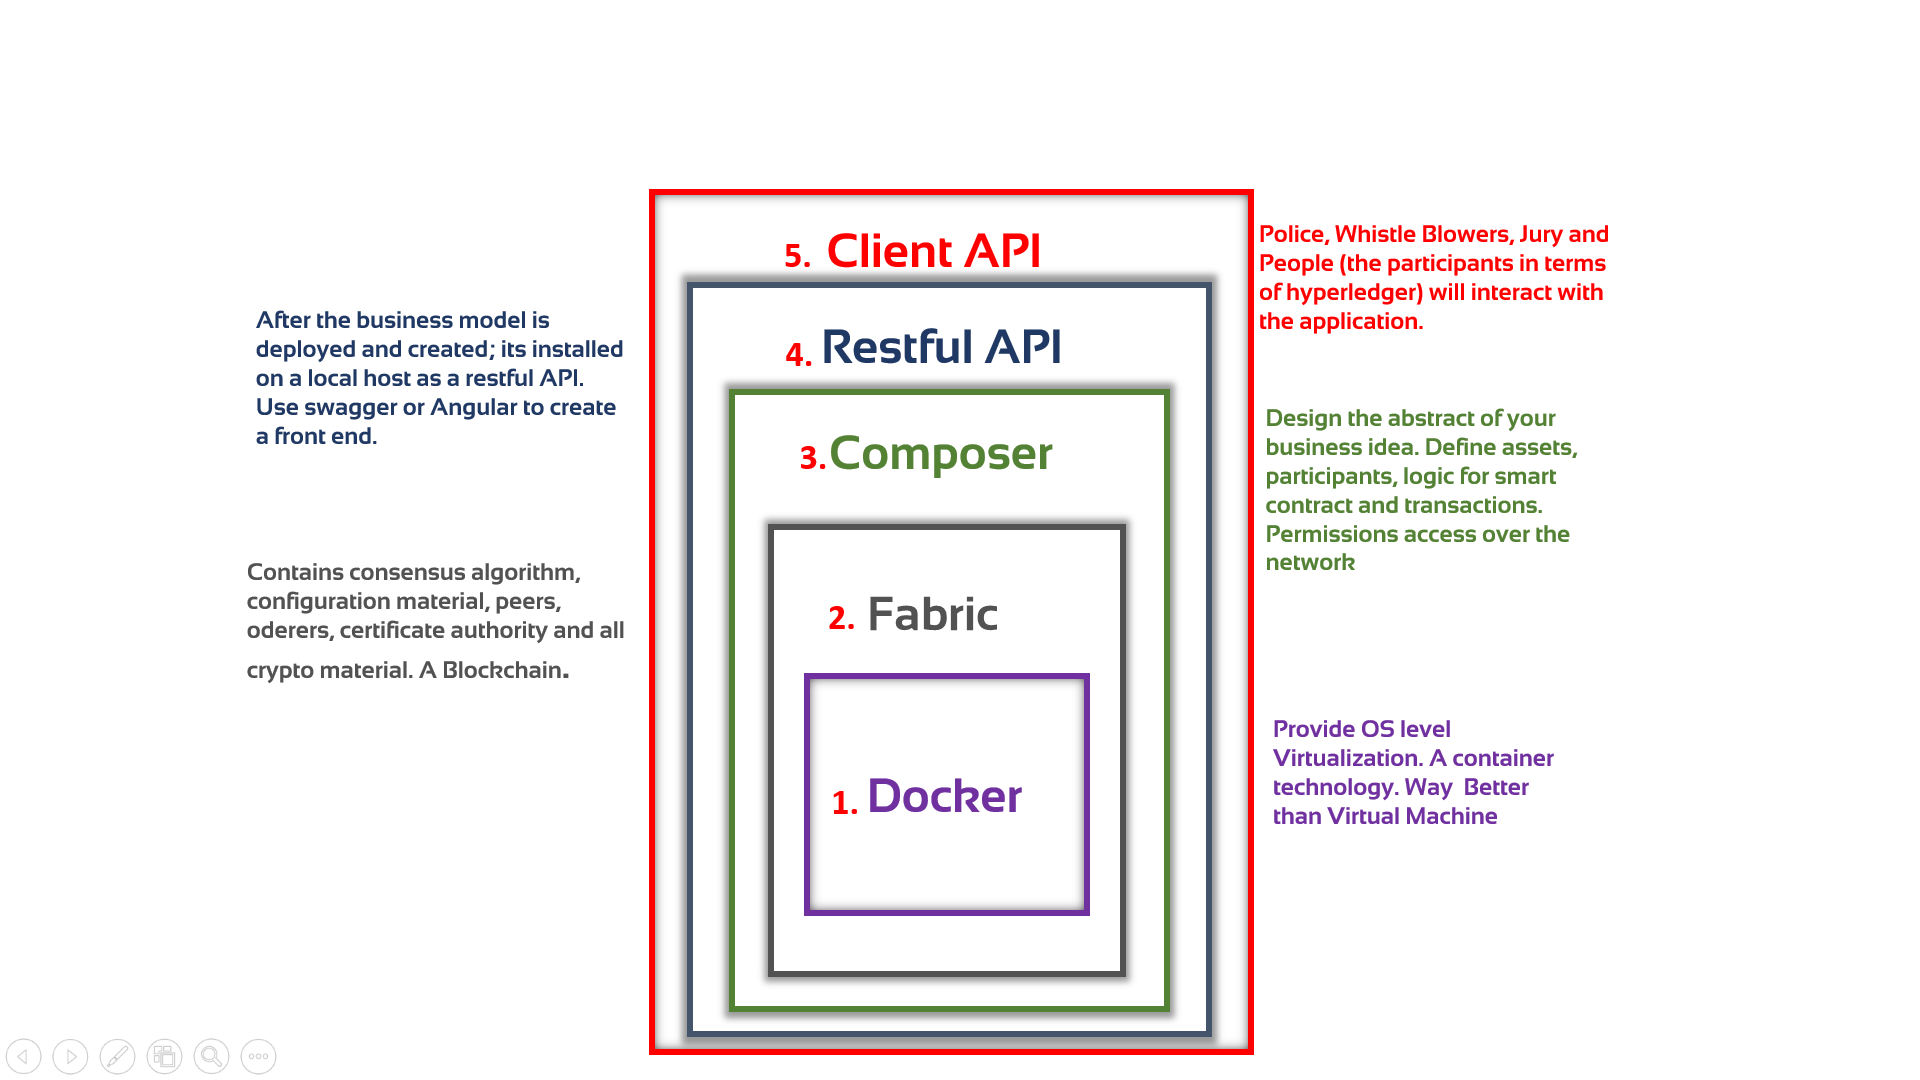
\includegraphics[scale=0.40]{figures/04.png}
	\caption{Blockchain }
	\label{fig:iste}
\end{figure}

\subsection{Hyperledger Fabric }
An open source undertaking grade per-mission circulated record innovation (DLT) stage, intended for use in big business settings, which conveys some key separating abilities over other famous appropriated record or blockchain stages. One key purpose of separation is that Hyperledger was set up under the Linux Foundation, which itself has a long and exceptionally effective history of supporting open source extends under open administration that become solid continuing networks and flourishing eco frameworks. \\
Hyperledger is administered by adverse specialized controlling advisory group, and the Hyperledger Fabric venture by a various arrangement of maintainers from numerous associations.\\ 
Texture is involved the accompanying measured parts:
\begin{itemize}
	\item A pluggable requesting administration builds up agreement on the request of exchanges and afterward communicates squares to peers.
	\item  A pluggable enrolment specialist co-op is in charge of partner elements in the system with cryptographic personalities.
	\item  A discretionary distributed babble benefit disperses the squares yield by requesting administration to different friends.
	\item  Savvy contracts ("chaincode") keep running inside a compartment domain (e.g. Docker) for separation. They can be written in standard programming dialects however don't have guide access to the record state.
	
\end{itemize}
\section{Hyperledger and Our Application }
\subsection{Hyperledger Composer}
It resembles a complier of Hyperledger Fabric. In arranger, we need to characterize our business organize. The exchanges and chain codes working. We here characterize our business organize rationale and test it on arranger play area before going ahead. \\
The fundamental parts of our Hyperledger Composer are.\\
\textbf{ Participants  }-One’s who is going to interact with the system. The Police, Whistle-Blower and the Jury.\\
\textbf{ 	Assets   }-Evidence and Cases. Any commodity which can be sold to the subscriber is an asset.\\
\textbf{ 	Transaction   }-The logic of chaincode responsible for validation and verification of every action happening on our blockchain.\\  
\textbf{ Query  }-To apply filters. Search specifically under given rates.\\
\textbf{ 	Permissions   }- An acl file to control read and write operation of participants over the network.
Combine together they make a .bna file which is later installed on a blockchain cloud.The figure below (see \figref{istg}) shows Hyperledger Architecture.\\
\begin{figure}[h]
	\centering
	\includegraphics[scale=0.40]{figures/05.png}
	\caption{Hyperledger Composer }
	\label{fig:istg}
\end{figure}
\subsection{IBM Cloud }
Cloud means a hosting service. Since it is not same as we host a simple website so we refer it as a blockchain cloud. The two main and famous clouds for hosting Hyperledger Blockchain Network are:

\begin{itemize}
	\item Amazon Web Services
	\item IBM Blockchain Cloud
	
\end{itemize}
These two platforms officially gives you an instance of Hyperledger Fabric which will interact with our .bna file.
Except that on every single Cloud Platform we have to manually install Hyperledger Fabric and Composer. Which will cost space and increase a lot of workload. We were testing IBM 
\subsection{Hyperledger Fabric}
Once the .bna file is created it has to interact with the Fabric.\\
Three main components of Hyperledger Fabric are: \\
\textbf{ Peer  }-The administrators are our friends which will embrace and perform agreement on arrangements.\\
\textbf{ Oderers  }-At whatever point a demand originate from endorser, to make it reach to companions and include it into blockchain arrange is its duty. Synchronization of correspondence on blockchain.\\
\textbf{Certificate Authority }-Gives administrator access to include peers create ssl endorsement and private and open keys for friends to maintain a strategic distance from breakdown and make netwoek secure. \\
As should be obvious in the image above once the IBM Blockchain Cloud account is made it straightforwardly gives you access to IBM Hyperledger Fabric Instance as every one of the three segments of Hyperledger Fabric are running, we simply need to introduce our .bna record in introduce code area.\\
\textbf{Channels }-We can make distinctive diverts in one blockchain arrange. We can likewise include diverse companions in that channel. One application is for one occasion inside that there are distinctive channels. 
Channels are utilized to have private correspondence.\\
For example you have private members you can add special peers and create separate chain for them.
\chapter{Interaction with Application
	\label{ch:Interaction with Application}}

A whistleblower is registering into the system, if it’s logging in to the system the Certificate Authority (CA) will look for its enrollment key in the hyperledger network and then grant him access to the network. Else the key will be put in the system while upon registering. 
\begin{itemize}
	\item	Enrollment Certificates and Transaction Certificates (E-certs and T-certs) can only be linked by CA and user. 
	\item 	Both the users will requests for certs. 
\end{itemize}
\textbf{Whistle Blower Sign up }-Access your Web page or Android application. Put up a \textbf{post }  request for  
registration and if it’s logging in, will put up a simple \textbf{ get } request that will retrieve your   
enrollment key from the blockchain application backend. The figure below (see \figref{istl}) shows Whistle Blower Sign up.\\ 
\begin{figure}[h]
	\centering
	\includegraphics[scale=0.90]{figures/06.png}
	\caption{Whistle Blower Sign up }
	\label{fig:istl}
\end{figure}  
The Hyperledger Fabric CA is a Certificate Authority (CA) for Hyperledger Fabric.\\
It provides features such as:
\begin{itemize}
	\item	registration of identities, or connects to LDAP as the user registry 
	\item 		issuance of Enrollment Certificates (ECerts)
	\item 		certificate renewal and revocation
\end{itemize}
The figure below (see \figref{istb}) shows Certificate Authority Architecture.\\ 
\begin{figure}[h]
	\centering
	\includegraphics[scale=0.90]{figures/07.png}
	\caption{Certificate Authority Architecture }
	\label{fig:istb}
\end{figure}  
\begin{itemize}
	\item	Interact with application
	\item 	Invoke the smart contract (Any request you put through)\\
	\textbf{      Updating Status }-Suppose you visited the after few days and a new evidence is found. If the case is solved, The Judge will change the status to solve. 
	\item 		Updating the distributed ledger 
		after the action will happen the distributed ledger will get updated. The consensus mechanism whether approve or disapprove your request a new block is added into the system.\\ 
		If the block is approved the world state of ledger will change else the world state will remain the same. 
	
\end{itemize}
The figure below (see \figref{istz}) shows Whole Whistle-blower Architecture.\\ 
\begin{figure}[h]
	\centering
	\includegraphics[scale=0.40]{figures/08.png}
	\caption{Whistle-blower Architecture }
	\label{fig:istz}
\end{figure}  
\section{Workflow of few Use Cases Together }
\subsection{Use Cases}
\subsubsection{Web Interface}
First you have to open the Front End of the application (Website) and see cases. Different cases will be uploaded there.
If you have any information regarding that you have to go and register on a whistle blower page
\subsubsection{Register a Whistle Blower}
It will not ask for your NIC or anything. You can register using a fake name and wallet. But in case you need reward wallet number can be put correctly and will not get trace back to you. One registration means one block is added into the system. Then you can submit an evidence to a case or report any illegal activity happening in the country.
\subsubsection{Discuss with Police}
The police can view all the cases and evidence and can submit their own. You can also discuss cases with the police and let’s see what their opinion about that case is. 
\subsubsection{Agency/Judge}
They are like few people 10-30 handling the system selected randomly to avoid them being get corrupted. The will also monitor police activities and their decisions over all the cases.  
\subsubsection{Blockchain Backend Working}
When a transaction is done all the peers node will see it and the consensus algorithm will take place. If it gets validated means the transaction is added in the ledger and it will change the world state of the blockchain.\\ 
If it’s not get validated it will still record that action that some subscriber tried this. It will be stored in the ledger but world state of blockchain is not updated.
The figure below (see \figref{istf}) shows the Work-flow diagram.\\ 
\begin{figure}[h]
	\centering
	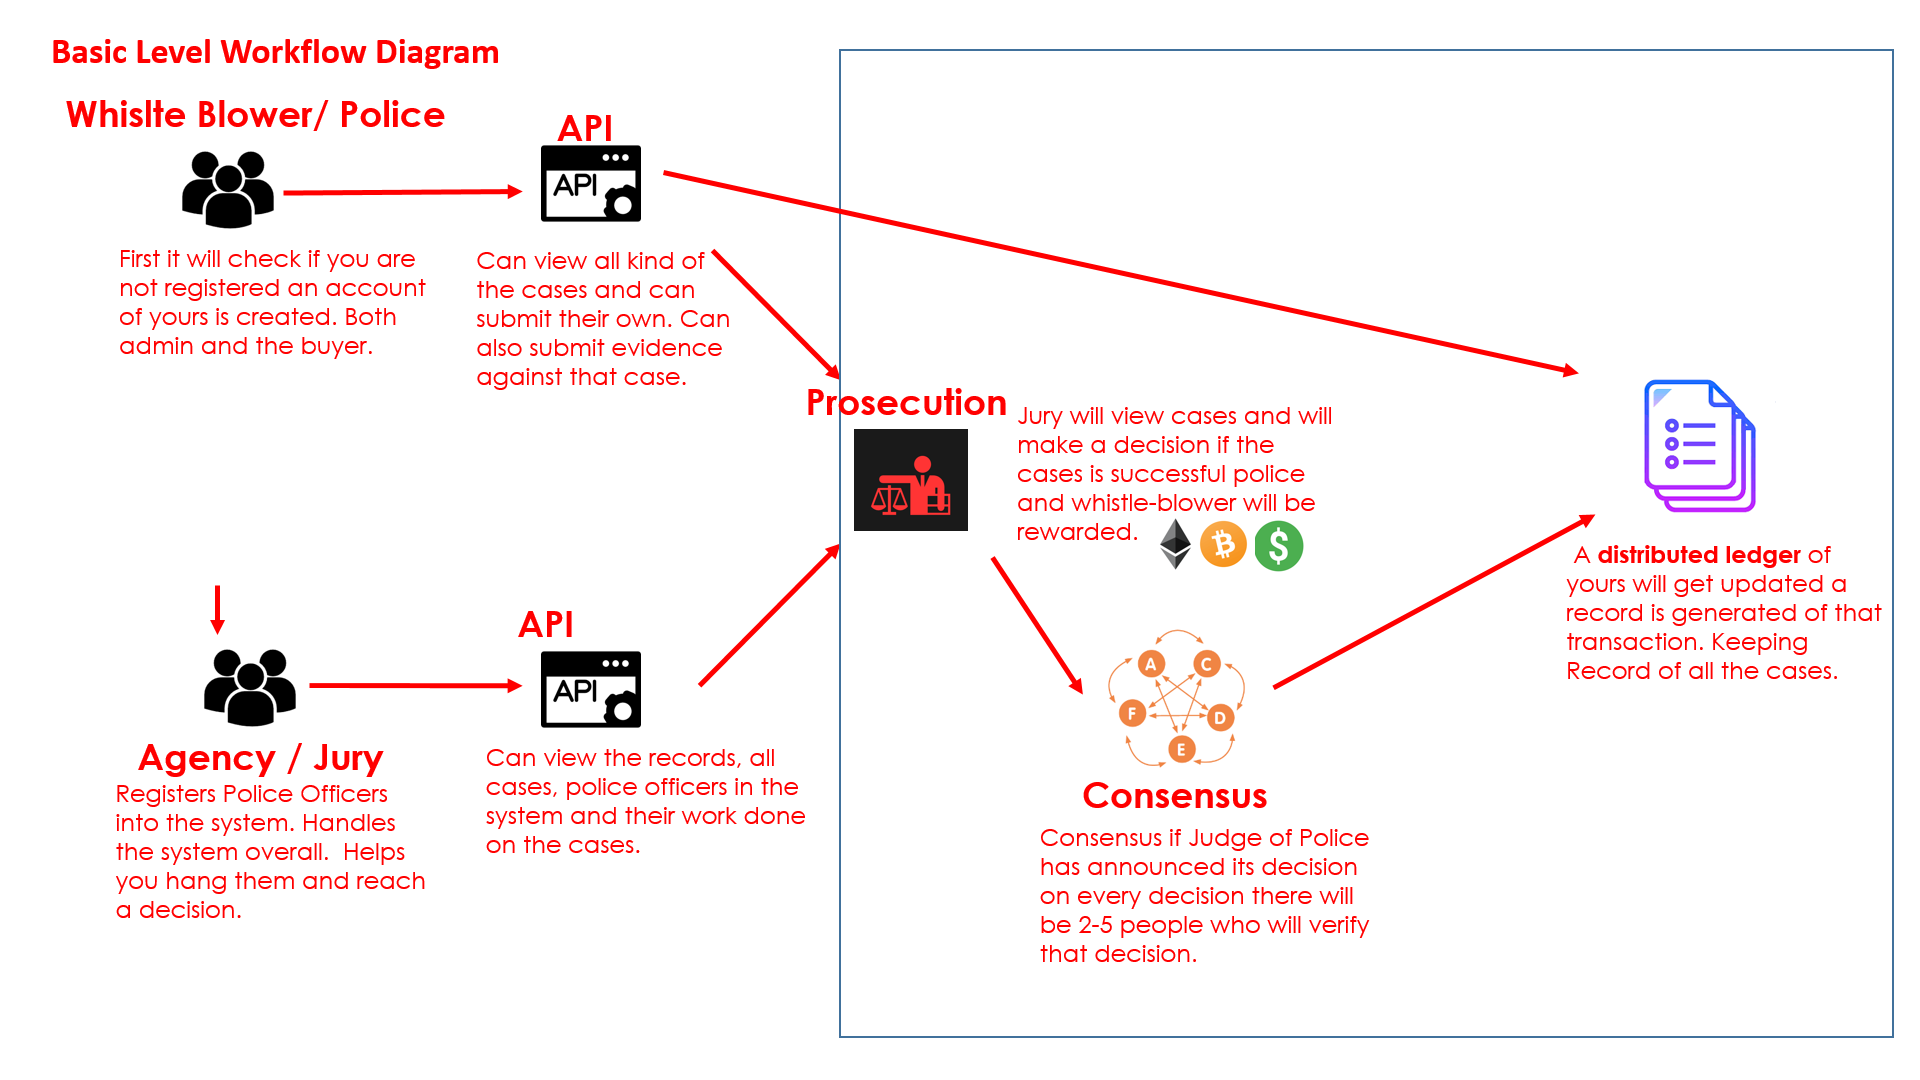
\includegraphics[scale=0.40]{figures/09.png}
	\caption{Work-flow diagram }
	\label{fig:istf}
\end{figure} 
\chapter{Installation And Configuration
	\label{ch:Installation And Configuration}}

In this chapter installation and configuration of \textbf{Hyperledger Composer }will be shown with dummy coding data.
The installation is for Ubuntu although Mac installation is also available if you are interested in that you can follow it on their official documentation on this Link.

\section{Installation}
\subsection{Pre-Requisites}
Open terminal by Ctrl+T and run these command. These will not run and ask you to install curl. Simply install curl and run this command.Make sure not to use sudo to run these commands.
\begin{figure}[h]
	\centering
	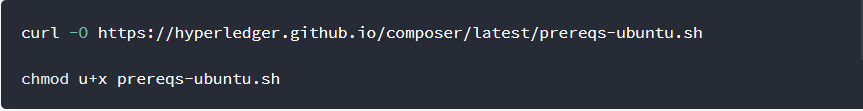
\includegraphics[width=450px]{figures/installation/1.png}
	
\includegraphics[width=450px]{figures/installation/2.png}
\end{figure}

The installation we have done above include textbf{Docker Node Git Python}
\subsection{Editor}
You can use whatever editor you want we recommend using \textbf{Visual Studio Code}.
\section{Installing Development Environment}
\subsection{Installing Command Line Tools}
\begin{figure}[h]
	\centering
	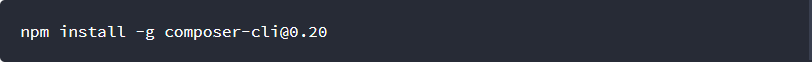
\includegraphics[width=450px]{figures/installation/3.png}
	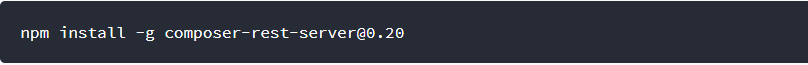
\includegraphics[width=450px]{figures/installation/4.png}
	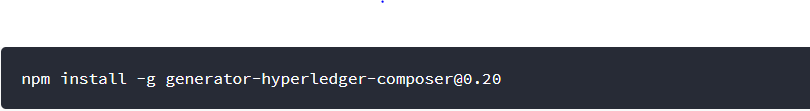
\includegraphics[width=450px]{figures/installation/5.png}
	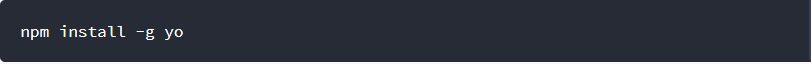
\includegraphics[width=450px]{figures/installation/6.png}
\end{figure}
\subsection{Installing Playground}
This is a playground tool for fabric in which you have to write the files (model, logic, permission, query)as discussed in the previous chapters 
\begin{figure}[h]
	\centering
	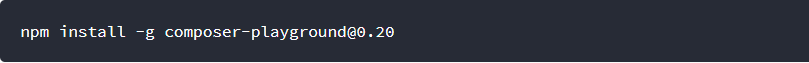
\includegraphics[width=450px]{figures/installation/7.png}
\end{figure}
\newpage
\subsection{Downloading Fabric}
\begin{figure}[h]
	\centering
	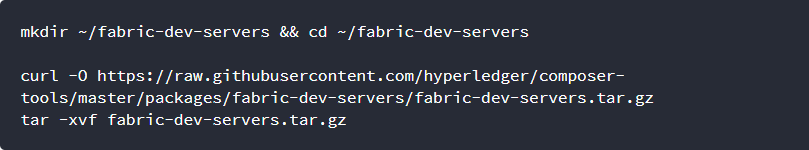
\includegraphics[width=450px]{figures/installation/8.png}
	\newline\newline
	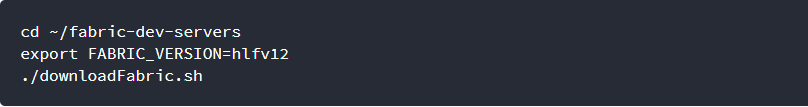
\includegraphics[width=450px]{figures/installation/9.png}

\end{figure}

Now the development installation is complete. \\To start fabric go to directory \textbf{fabric-dev-servers} and use this command.\\
\textbf{./startFabric.sh}
\\To stop fabric use this command inside the same directory.\\
\textbf{./stopFabric.sh}
\\And to open playground in the browser use any where in the terminal. \\
\textbf{composer-playground}
\\make sure not to use \textbf{sudo} with these commands.
\\Congratulations you have completed all installation now we will move on deployment.

\section{Deployment of Composer}
\begin{itemize}
	\item Open the composer playground and click on \textbf{Deploy a new business network}
	\item Name your business network 
	\item Select empty-business-network
	\item Now click on Deploy
\end{itemize}
Once the network is deployed connect to it. After connecting to network you have to add / write your files here.
\subsection{Adding Model File}
\begin{itemize}
	\item Click on \textbf{Model File} to view it, delete the code written there and add the following in there
\end{itemize}
\begin{figure}[h]
	\centering
	\includegraphics[width=450px]{figures/installation/10.png}
\end{figure}
\newpage
\subsection{Adding your Logic File}
\begin{itemize}
	\item Click on add file and choose script file
	\item Delete the code and add the following code
\end{itemize}

\begin{figure}[h]
	\centering
	\includegraphics[width=450px]{figures/installation/11.png}
\end{figure}
This is enough for testing the deployment of fabric.
\section{Deployment of business network}
\subsection{Creating business network structure}
Run this command 
\begin{figure}[h]
	\centering
	\includegraphics[width=450px]{figures/installation/12.png}
\end{figure}

\subsection{Generating business network archive}
Run this command 
\begin{figure}[h]
	\centering
	
\includegraphics[width=450px]{figures/installation/13.png}
\end{figure}

\subsection{Installing business network}
Run this command 
\begin{figure}[h]
	\centering
	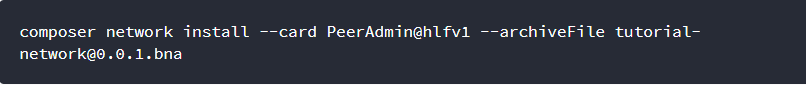
\includegraphics[width=450px]{figures/installation/14.png}
\end{figure}

\subsection{Starting business network}
Run this command 
\begin{figure}[h]
	\centering
	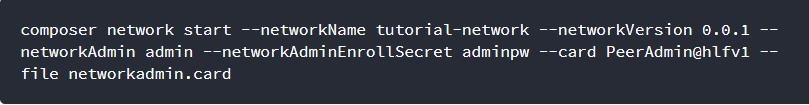
\includegraphics[width=450px]{figures/installation/15.png}
\end{figure}
\subsection{Importing network administrator card}
Run this command 
\begin{figure}[h]
	\centering
	
\includegraphics[width=450px]{figures/installation/16.png}
\end{figure}
\newpage
\section{Genrating rest server}

Run this command. 
\begin{figure}[h]
	\centering
	
\includegraphics[width=450px]{figures/installation/18.png}
\end{figure}\\
You will be asked to give 
\begin{itemize}
	\item Network card name. 
	\item Select never use namespaces
	\item After that select textbf{No} to everything
\end{itemize}




\chapter{InterPlanetary File System
	\label{ch:InterPlanetary File System}}

The \textbf{Interplanetary File System} is a protocol and network designed to create a content-addressable, peer-to-peer method of storing and sharing hypermedia in a distributed file system. IPFS is a peer-to-peer distributed file system that seeks to connect all computing devices with the same system of files.
\section{IPFS Working}
In the figure below (see \figref{ipfs1}) shows an example of a person name jon who want to send a file using \textbf{IPFS}. By using \textbf{IPFS} File would be convert into \textbf{Hash} that would upload in InterPlanetary File System. 


\begin{figure}[h]
	\centering
	\includegraphics[width=450px]{figures/IPFS/10.png}
	\caption{IPFS File Upload}
	\label{fig:ipfs1}
\end{figure}

When Another Person name Sky want to Access that file just use \textbf{Hash} in InterPlanetary File System that give permission to Sky 
when \textbf{Hash} would match that upload in InterPlanetary File System see  the figure below (see \figref{ipfs2}) shows an example of Sky who Access that File.

\begin{figure}[h]
	\centering
	\includegraphics[width=450px]{figures/IPFS/11.png}
	\caption{IPFS File Access}
	\label{fig:ipfs2}
\end{figure}

IPFS would be same as BlockChain Network. When a File would be upload it turn on the Security that would not be Hacked the figure below (see \figref{ipfs3}) shows if Hash was Right file would be Access otherwise not Access-able. 
\begin{figure}[h]
	\centering
	\includegraphics[width=450px]{figures/IPFS/12.png}
	\caption{IPFS File Access}
	\label{fig:ipfs3}
\end{figure}


\section{Installation}
\subsection{Install IPFS}
First of all install IPFS from their offical site that would be shown below.

\begin{figure}[h]
	\centering
	\includegraphics[width=450px]{figures/IPFS/01.png}
\end{figure}

\subsection{Editor}
You can use whatever editor you want we recommend using \textbf{Visual Studio Code} where we Attach \textbf{IPFS API} with \textbf{React}.
\newpage
\section{IPFS Update}
\subsection{Installing with IPFS-Update}
The Below figure shows IPFS-Updation
\begin{figure}[h]
	\centering
	\includegraphics[width=450px]{figures/IPFS/02.png}
	\includegraphics[width=450px]{figures/IPFS/04.png}
	
\end{figure}

\section{IPFS Repository}
\subsection{Initialize the repository}
IPFS stores all its settings and internal data in a directory called the repository. Before using IPFS for the first time, you’ll need to initialize the repository with the \textbf{ ipfs init} command The Below figure shows IPFS-Repository
\begin{figure}[h]
	\centering
	\includegraphics[width=450px]{figures/IPFS/05.png}
\end{figure}

Now, try running the command suggested to you in the output of ipfs init. The one that looks like \textbf{ipfs cat /ipfs/<HASH>/readme}.
You get Something like that show below
\begin{figure}[h]
	\centering
	\includegraphics[width=310px]{figures/IPFS/06.png}
	\includegraphics[width=310px]{figures/IPFS/09.png}
\end{figure}
\newpage
These steps can install your IPFS. Now for Check you can upload a hash using  (see \figref{ipfs7})

\begin{figure}[h]
	\centering
	\includegraphics[width=450px]{figures/IPFS/07.png}
	\caption{Upload Hash}
	\label{fig:ipfs7}
\end{figure}

When we Check our File that Upload in IPFS you can use same hash using (see \figref{ipfs8}) in Command line.
\begin{figure}[h]
	\centering
	\includegraphics[width=450px]{figures/IPFS/08.png}
	\caption{Get Hash}
	\label{fig:ipfs8}
\end{figure}
\chapter{Reward System
	\label{ch:Reward System}}

The \textbf{Reward System} is the last step of Whistle-Blower Application that would be implemented in \textbf {Ethereum Crypto-Currency}.\newline
Reward System is Used for Whistle-Blower when he Upload case and after inquiry the case status would be completed then government make a threshold for Reward in Ethereum that would be Transfer to Whistle-Blower Account after case Complete.    
\section{Ethereum}
\textbf {Ethereum} is an open-source, open, blockchain-based disseminated figuring stage and working framework including savvy contract usefulness. It bolsters an adjusted form of Nakamoto accord by means of exchange based state changes. Ether is a token whose blockchain is produced by the Ethereum stage. 
Ethereum Provides a Platform for Developers to make
Decentralized Application.It Facilitate the Exchange of Money, Property and many
more.
\subsection{Ethereum VS Bitcoin}
The structure of the ethereum blockchain is fundamentally the same as bitcoin's, in that it is a mutual record of the whole exchange history. Each hub on the system stores a duplicate of this history. 

The huge distinction with ethereum is that its hubs store the latest condition of each savvy contract, notwithstanding the majority of the ether exchanges. (This is significantly more entangled than depicted, yet the content beneath should enable you to get your feet wet.) 

For each ethereum application, the system needs to monitor the 'state', or the present data of these applications, including every client's parity, all the keen contract code and where it's everything put away. 

Bitcoin utilizes unspent exchange yields to follow who has how much bitcoin. 

While it sounds increasingly unpredictable, the thought is genuinely basic. Each time a bitcoin exchange is made, the system 'breaks' the aggregate sum as though it was paper cash, issuing back bitcoins such that influences the information to act likewise to physical coins or change. 

To make future exchanges, the bitcoin organize must include every one of your bits of progress, which are classed as either 'spent' or 'unspent'. 

Ethereum, then again, utilizes accounts. 

Like financial balance reserves, ether tokens show up in a wallet, and can be ported (as it were) to another record. Assets are in every case some place, yet don't have what you may call a proceeded with relationship.
\begin{figure}[h]
	\centering
	\includegraphics[width=300px]{figures/Ethereum/02.png}
	\caption{Ethereum vs Bitcoin}
	\label{fig:ipfs1}
\end{figure}
\newpage
\subsection{Ethereum Working}
With ethereum, each time a program is utilized, a system of thousands of PCs forms it. 

Contracts written in a brilliant contract-explicit programming dialects are gathered into 'bytecode', which an element called the 'ethereum virtual machine' (EVM) can peruse and execute. 

Every one of the hubs execute this agreement utilizing their EVMs.
\begin{figure}[h]
	\centering
	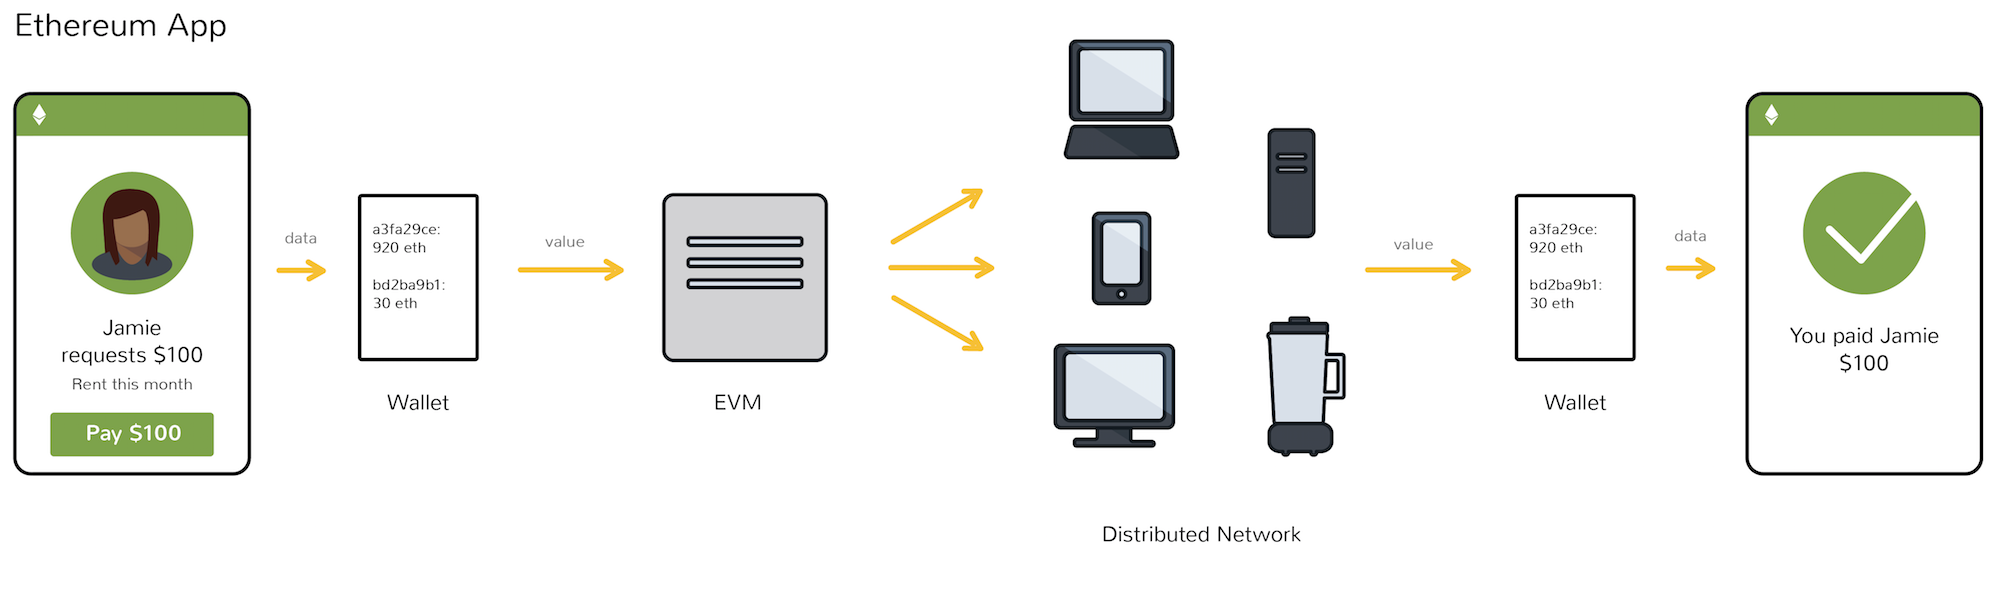
\includegraphics[width=450px]{figures/Ethereum/01.png}
	\caption{Ethereum Working}
	\label{fig:ipfs1}
\end{figure}

Keep in mind that each hub in the system holds a duplicate of the exchange and savvy contract history of the system, notwithstanding monitoring the current 'state'. Each time a client plays out some activity, the majority of the hubs on the system need to come to understanding that this change occurred. 

The objective here is for the system of excavators and hubs to assume liability for exchanging the move from state to state, instead of some expert, for example, PayPal or a bank. Bitcoin excavators approve the move of responsibility for starting with one individual then onto the next. The EVM executes an agreement with whatever administers the engineer at first modified. 

Real calculation on the EVM is accomplished through a stack-based bytecode language (the zeroes that a machine can peruse), however designers can compose keen contracts in abnormal state dialects, for example, Solidity and Serpent that are simpler for people to peruse and compose. 

As clarified in our guide "How Ethereum Mining Works", excavators are the ones that are anticipating awful conduct – like guaranteeing that nobody is spending their cash more than once and dismissing brilliant contracts that haven't been paid for. 

There are a couple of thousand ethereum hubs out there, and each hub is arranging and executing a similar code.


\subsection{Smart Contract In Ethereum}
It's significant that bitcoin was the first to help fundamental shrewd contracts as in the system can exchange an incentive starting with one individual then onto the next. The system of hubs will possibly approve exchanges if certain conditions are met. 
\begin{figure}[h]
	\centering
	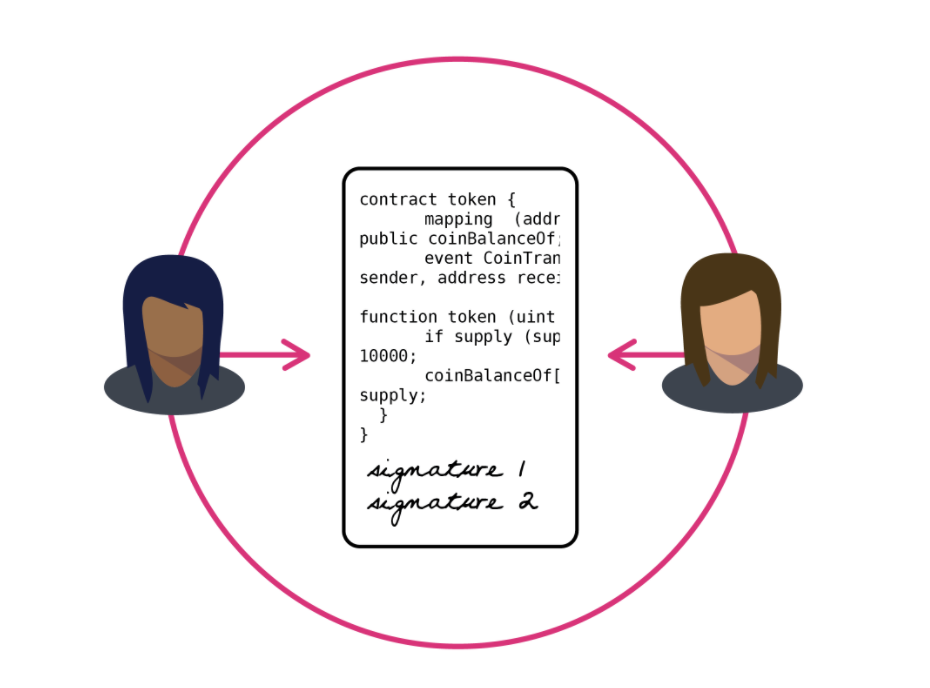
\includegraphics[width=300px]{figures/Ethereum/03.png}
	\caption{Ethereum Smart Contract}
	\label{fig:ipfs1}
\end{figure}
However, bitcoin is constrained to the cash use case. 

On the other hand, ethereum replaces bitcoin's increasingly prohibitive language (a scripting language of a hundred or so contents) and replaces it with a language that enables engineers to compose their very own projects. 

Ethereum enables engineers to program their very own savvy contracts, or 'self-ruling specialists', as the ethereum white paper calls them. The language is 'Turing-finished', which means it bolsters a more extensive arrangement of computational directions.

Shrewd contracts can: 
\begin{itemize}
	\item Capacity as 'multi-signature' accounts, with the goal that reserves are spent just when a required level of individuals concur 
	\item Oversee understandings between clients, state, on the off chance that one purchases protection from the other
	\item Give utility to different contracts (like how a product library works) 
	
	\item Store data around an application, for example, area enlistment data or participation records.
\end{itemize}

\newpage
\section{Ethereum Installation and Integration}
\subsection{Background}
First we should know how our project will interact with the ethereum blockchain. To demonstrate that lets have a look at the picture below.
\begin{figure}[h]
	\centering
	\includegraphics[width=300px]{figures/Ethereum/04.png}
	\caption{Broader View of Ethereum}
	\label{fig:eth4}
\end{figure}

\subsection{Metamask Wallet}
The right block of the diagram shows ethereum nodes and left blocks shows how we can interact with the ethereum network/nodes.Developers uses web3.js library to interact with this ethereum network. Customers/consumers uses Metamask, a browser extention or Mist browser to play with contracts written in ethereum.\\
Metamask provides an ethereum wallet which consists of an account address, public key and a private key. Which can be used for all the four networks provided by ethereum. \textbf{Main} network is ethereum real network and rest of three are for testing purposes.
\begin{figure}[h]
	\centering
	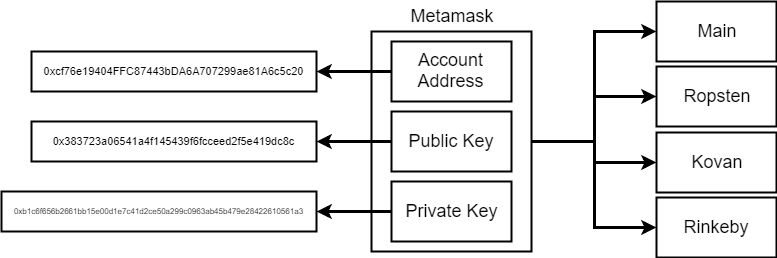
\includegraphics[width=300px]{figures/Ethereum/05.png}
	\caption{Metamask Wallet Structure}
	\label{fig:eth5}
\end{figure}

\subsection{Transaction Structure}
Following bewlow picture demonstrates parameters of a transaction that are required to do a transaction in any ethereum network.
\begin{figure}[h]
	\centering
	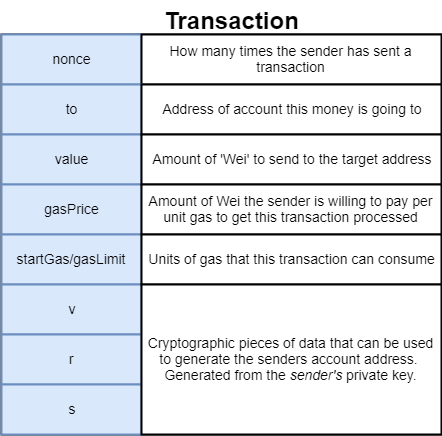
\includegraphics[width=300px]{figures/Ethereum/06.png}
	\caption{Ethereum Transaction Structure}
	\label{fig:eth6}
\end{figure}

\subsection{Installation}
Writing contracts in ethereum needs following things.
\begin{itemize}
	\item  Solidity Compiler
	\item  Local or Test Network (Ganache)
\end{itemize}

For writing Contracts in ethereum we'll be using solidity programming language. To compile its code we use solidity compiler. For testing our contracts before deploying our contract to main network we'll be using \textbf{Ganache}.
\newpage 
First we need to create a folder and install the following tools.
\begin{itemize}
	\item  run command " npm init "
	\item  Install solidity compiler by running command " npm install --save solc@0.4.17 "
	\item  Installing local network for ethereum by running command  
	" npm install --save mocha ganache-cli "
\end{itemize}
Stucture of your folder should be as figure below. package.jason file will be added by running npm init command.
\begin{figure}[h]
	\centering
	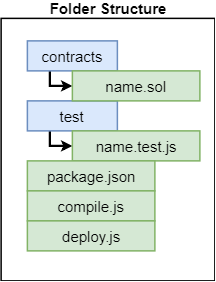
\includegraphics[width=300px]{figures/Ethereum/08.png}
	\caption{Folder Structure}
	\label{fig:eth7}
\end{figure}\newpage

Good to go now you can write your contracts. When contracts are compiled by solidity compiler it gives us its ABI (application binary interface) and contract bytecode. 
\begin{figure}[h]
	\centering
	\includegraphics[width=300px]{figures/Ethereum/09.png}
	\caption{Folder Structure}
	\label{fig:eth7}
\end{figure}
\\Our main concern is with the bytecode that is given after compiling by solidity compiler. This bytecode will be used to deploy contracts on our local, test or infact main ethereum network. And ABI will be used by web3.js so that we can interact or write useful fron-ends.
\chapter{Conclusions and Future Work}

\section{Conclusion}
The corruption is increasing day by day. People don’t know who to trust. Every other person in your neighborhood can be working for another person. Building a network topology of people or group of people called mafia is threatening the peace keepers and well-wishers of the society. The best people of society don’t know who to trust. From a simple staff employee to the highest level of the Government Official can be involved in this. The whistle blowers that are reporting or planning on reporting don’t even know who they are talking to. The crime rate in Pakistan is increasing day by day. They are afraid of getting themselves killed or hurt.\\
The Solution to report crime or any illegal activity happening in the country safely is that we develop a blockchain based reward system for whistle blowers where the identities of the Police Officer and the whistle blowers kept safely.\\
The Basic Structure of the application is discussed below:\\
\textbf{The Smart Contract  }-An electronic contract in the blockchain application where the trade is happening when whistle blower reports something and gets rewarded.\\ 
\textbf{The Police }-Will submit both cases and evidence against any case uploaded by any whistle blower or any other police officer. Can view both cases and evidence of any region in the country.\\
\textbf{The People  }-The people will see all the cases up and running currently. If you have anything against any case you have to register on a whistle blower page. \\
\textbf{The Whistle-Blower  }-– Instead of real name or anything they will register through a wallet number. Keeping them unknown to the police and everyone on the system. They can submit both the cases and the evidence against any case.\\
\textbf{The Agency/Judge  }-– They will keep an eye on the cases and officer assigned to that case. Reward them both the officer and the whistle blower for successful closing of the case.\\
The Solution aims to build as many use cases as possible regarding this application. Ensuring the safety of whistle blowers is our first priority. That’s why we used their wallets number to register them instead of their names. The cases older than 3 months will get dispose into another forum.\\ 
Make this prototype as a working model as soon as possible and to get hold and reduce crime rate happening in our country is our main goal. Thanks to our Government and President enthusiasm to take action against crime and involving technology for the safety of good people in our society means a lot to us.  


%\appendix
% \chapter{Appendix I title}
 
 text here


\bibliographystyle{plain}
\bibliography{bib} 
\addcontentsline{toc}{chapter}{References} 

\end{document}
